\chapter{Diseños de Pantallas}
	\label{diseños}
	\noindent Este apartado, se muestran los diseños de pantallas que se consideraron para incluir en el proyecto final. Se muestran los distintos módulos de cada uno de los participantes involucrados en la aplicación web.
	
		\begin{figure}[hbt!]
			\centering
			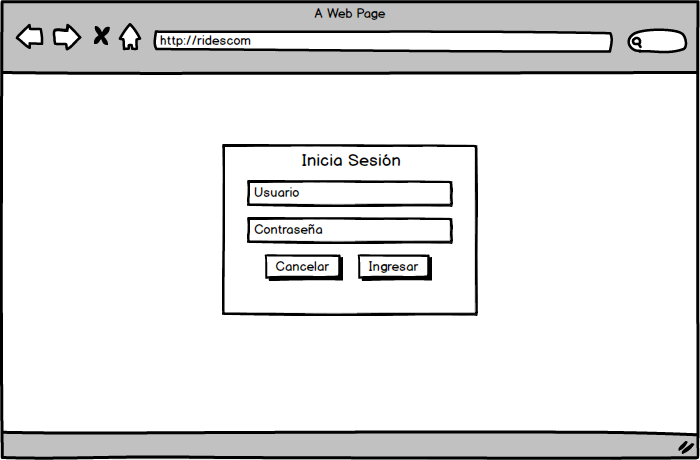
\includegraphics[width=10cm, height=6cm]{Imagenes/Nuevos/P1_LoginJFD_coord}
			\caption{Inicio sesión para el JFD y el coordinador de U.A.}
			\label{inicioJFDycoord}
		\end{figure}
		\pagebreak
		
		\begin{figure}[hbt!]
			\centering
			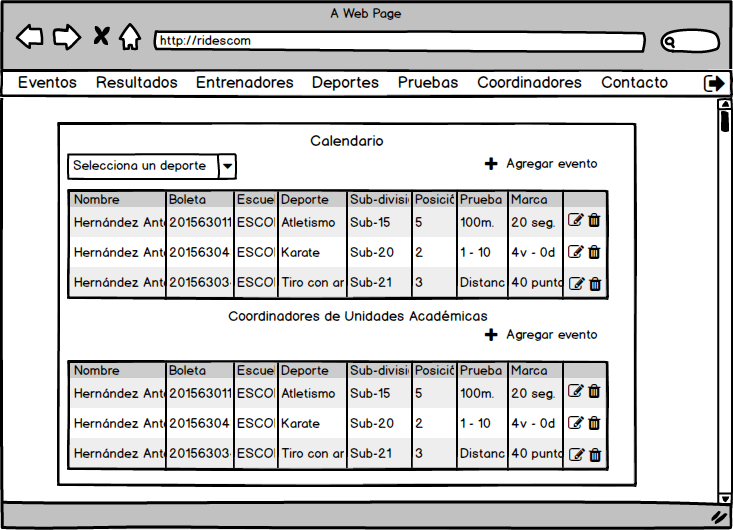
\includegraphics[width=10cm, height=6cm]{Imagenes/Nuevos/P2_Inicio_JefeFD}
			\caption{Página principal para el Jefe de Fomento Deportivo}
			\label{principalJFD}
		\end{figure}
	
		\begin{figure} [hbt!]
			\centering
			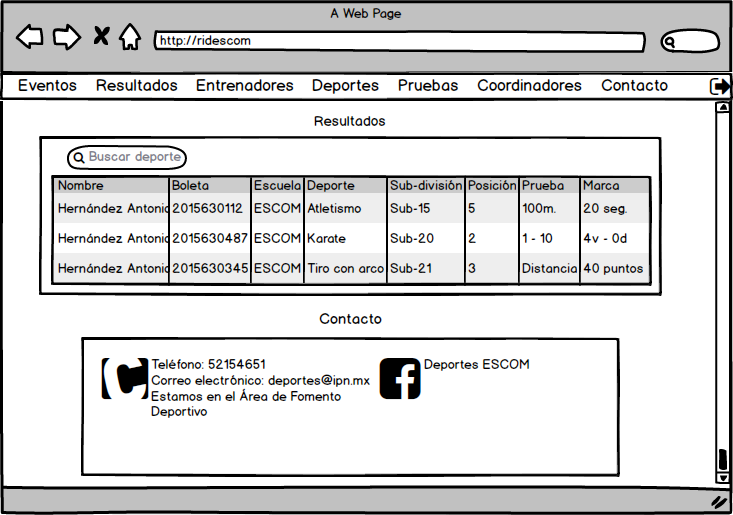
\includegraphics[width=10cm, height=6cm]{Imagenes/Nuevos/P3_Inicio_JefeFD1}
			\caption{Página principal para el Jefe de Fomento (Continuación).}
			\label{principalJFD1}
		\end{figure}
	
		\begin{figure} [hbt!]
			\centering
			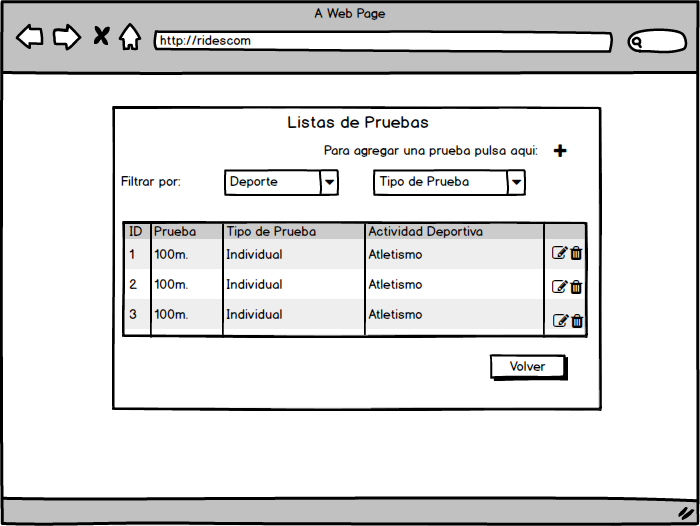
\includegraphics[width=10cm, height=6cm]{Imagenes/Nuevos/P25_Pruebas_JFD}
			\caption{Página para visualizar las pruebas dadas de alta. (Jefe de Fomento Deportivo)}
			\label{pruebas}
		\end{figure}
		\pagebreak
		
		\begin{figure} [hbt!]
			\centering
			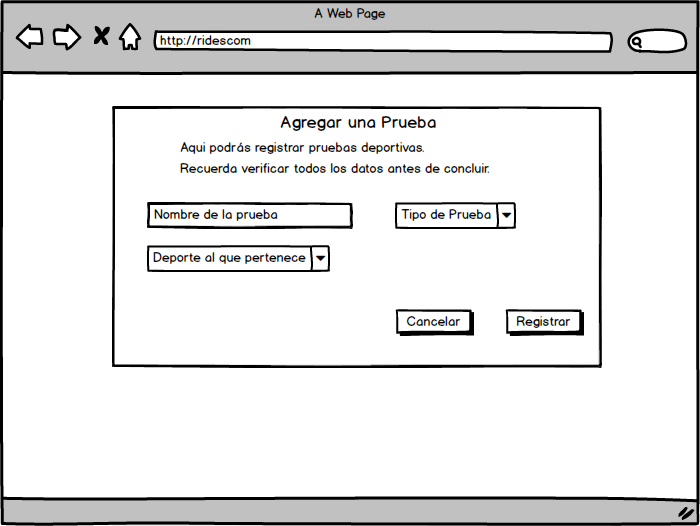
\includegraphics[width=10cm, height=6cm]{Imagenes/Nuevos/P26_AgregarPruebas_JFD}
			\caption{Página para agregar las distintas pruebas pruebas. (Jefe de Fomento Deportivo)}
			\label{agregarpruebas}
		\end{figure}
		
		\begin{figure} [hbt!]
			\centering
			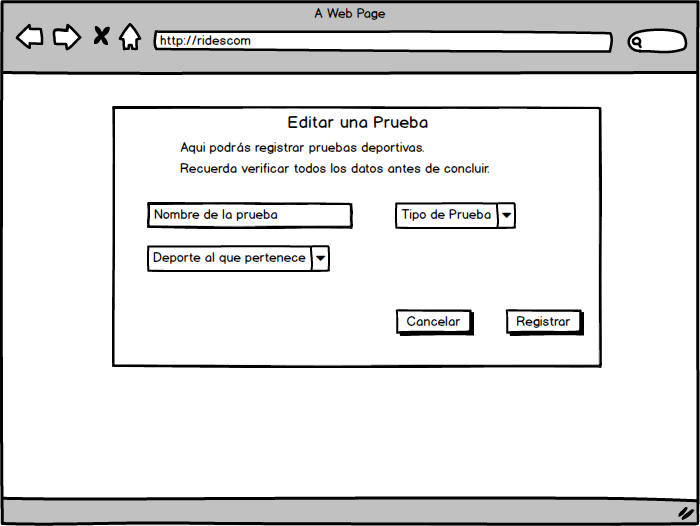
\includegraphics[width=10cm, height=6cm]{Imagenes/Nuevos/P26_EditarPruebas_JFD}
			\caption{Página para editar los datos de las pruebas previamente registrados. (Jefe de Fomento Deportivo)}
			\label{editarpruebas}
		\end{figure}
	
		\begin{figure} [hbt!]
			\centering
			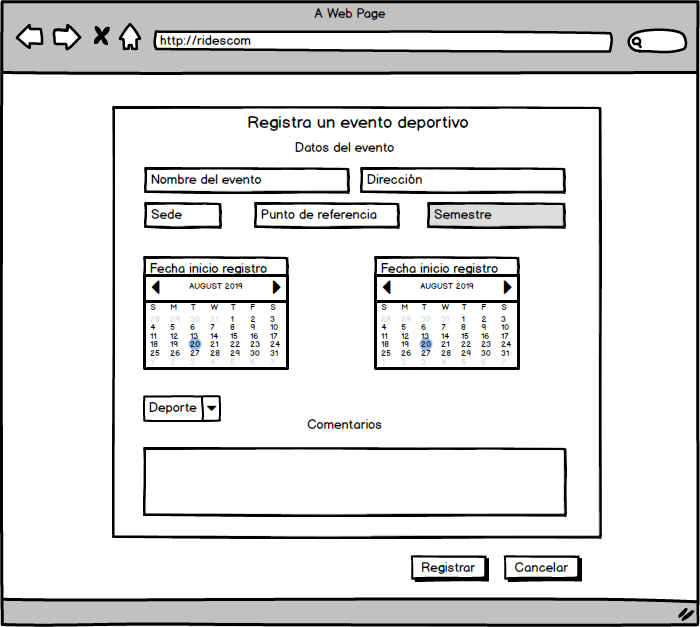
\includegraphics[width=10cm, height=6cm]{Imagenes/Nuevos/P4_Crear_evento_deportivo}
			\caption{Vista para dar de alta un evento deportivo (Jefe de Fomento Deportivo).}
			\label{creaevento}
		\end{figure}
		\pagebreak	
		
		\begin{figure} [hbt!]
			\centering
			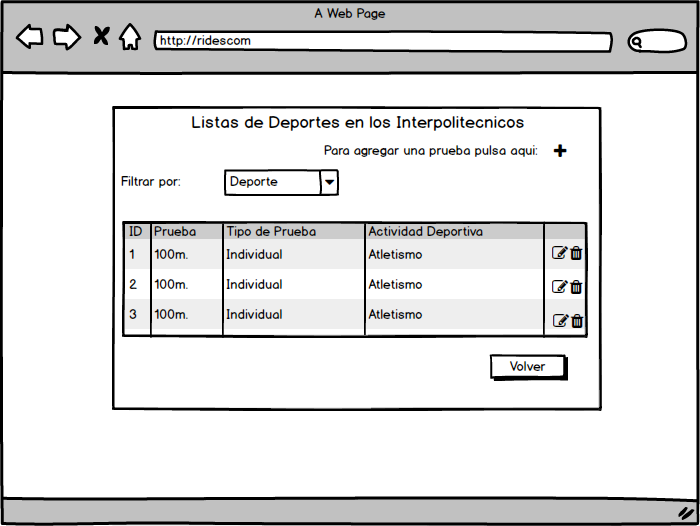
\includegraphics[width=10cm, height=6cm]{Imagenes/Nuevos/P27_Deportes_JFD}
			\caption{Página para visualizar los deportes que se llevaran a cabo en los eventos interpolitécnicos}
			\label{deportes}
		\end{figure}
	
		\begin{figure} [hbt!]
			\centering
			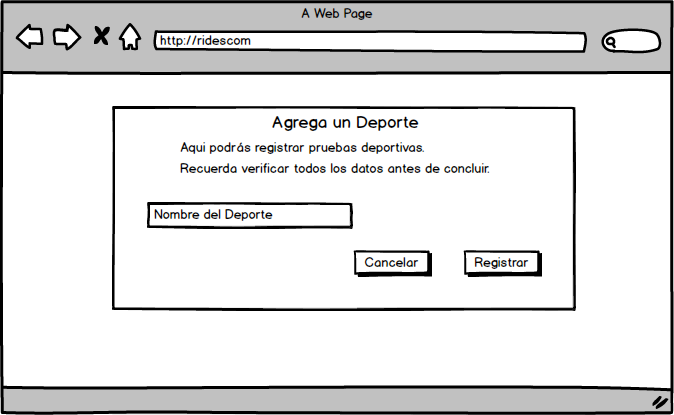
\includegraphics[width=10cm, height=6cm]{Imagenes/Nuevos/P28_AgregarDeportes_JFD}
			\caption{Página para agregar un deporte.}
			\label{agregadeporte}
		\end{figure}
		
		\begin{figure} [hbt!]
			\centering
			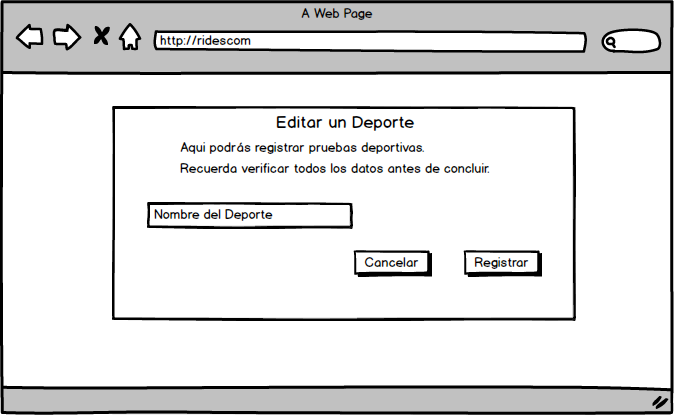
\includegraphics[width=10cm, height=6cm]{Imagenes/Nuevos/P29_EditarDeportes_JFD}
			\caption{Página para editar datos de los deportes}
			\label{editardeporte}
		\end{figure}
		\pagebreak
		
		\begin{figure} [hbt!]
			\centering
			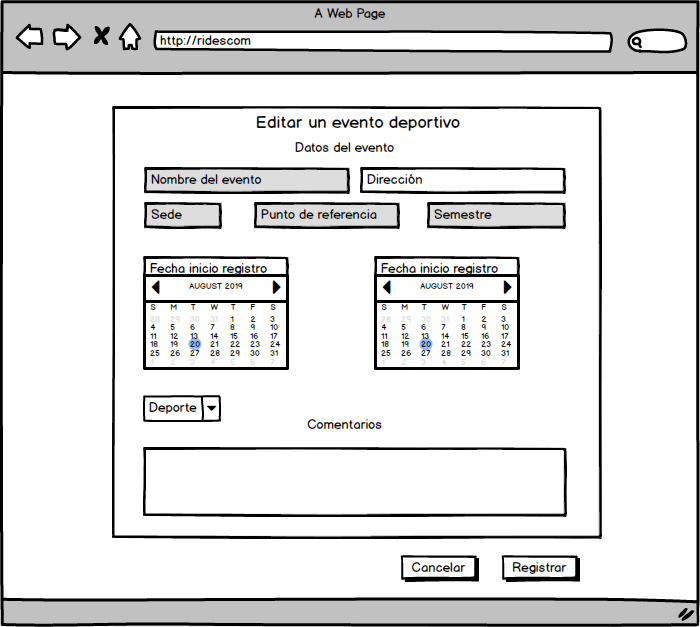
\includegraphics[width=10cm, height=6cm]{Imagenes/Nuevos/P5_Editar_evento_deportivo}
			\caption{Vista para editar datos de un evento ya registrado. (Jefe de FOmento Deportivo).}
			\label{editarevento}
		\end{figure}
	
		\begin{figure} [hbt!]
			\centering
			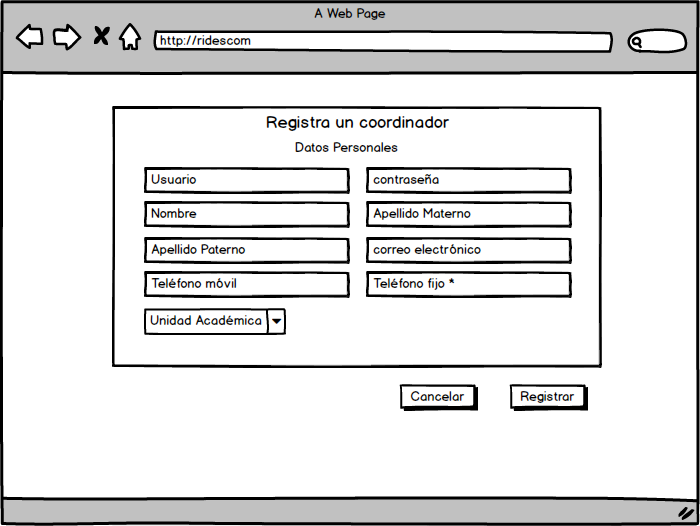
\includegraphics[width=10cm, height=6cm]{Imagenes/Nuevos/P6_Registro_coordinador}
			\caption{Vista para registrar un coordinador de unidad académica. (Jefe de Fomento Deportivo).}
			\label{registrarcoord}
		\end{figure}
		
		\begin{figure} [hbt!]
			\centering
			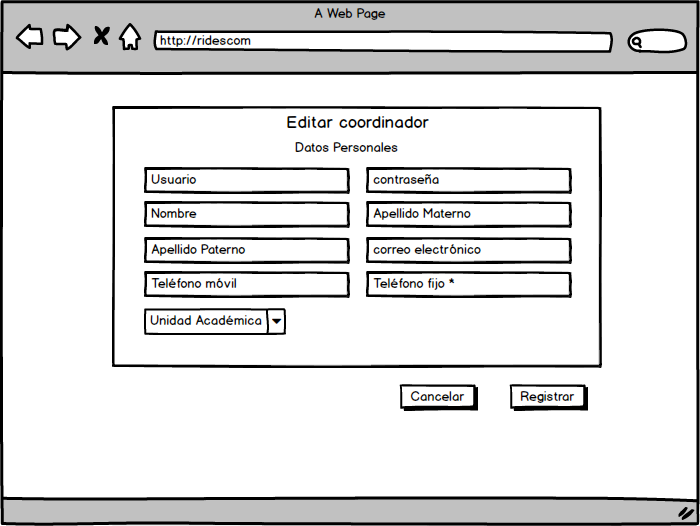
\includegraphics[width=10cm, height=6cm]{Imagenes/Nuevos/P7_Editar_coordinador}
			\caption{Vista para editar datos de un coordinador previamente registrado. (Jefe de Fomento Deportivo).}
			\label{editarcoord}
		\end{figure}
\pagebreak

		\begin{figure} [hbt!]
			\centering
			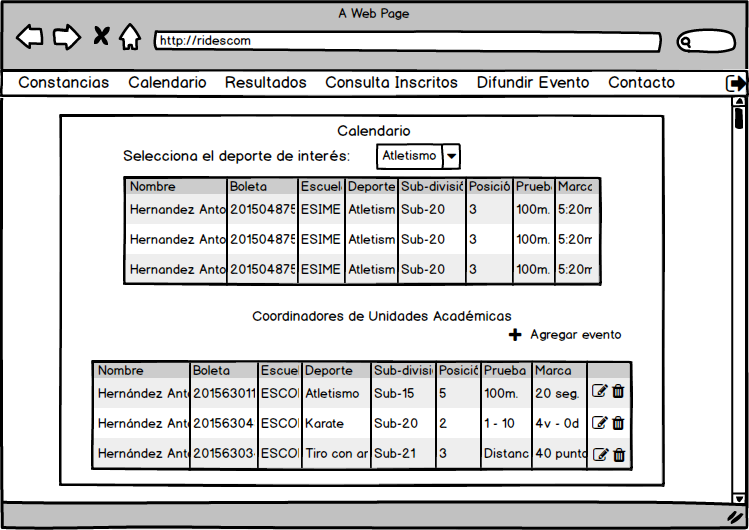
\includegraphics[width=10cm, height=6cm]{Imagenes/Nuevos/P8_Inicio_CoordUA}
			\caption{Vista principal para el coordinador de una Unidad Académica.}
			\label{principalcoord}
		\end{figure}
	
		\begin{figure} [hbt!]
			\centering
			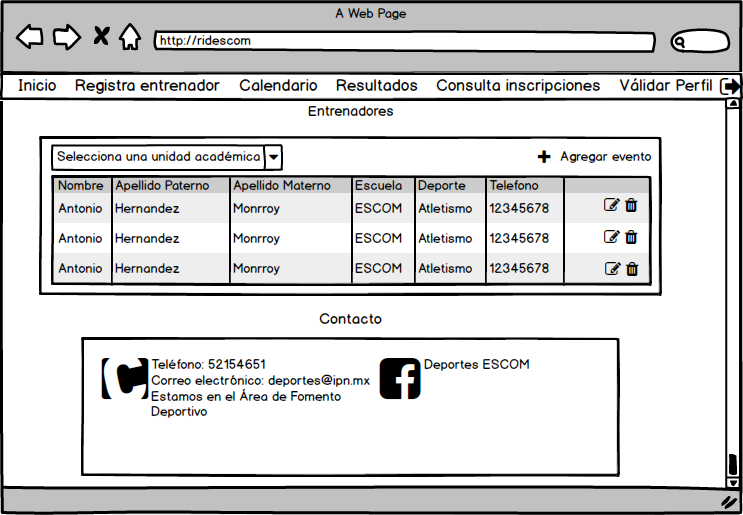
\includegraphics[width=10cm, height=6cm]{Imagenes/Nuevos/P9_Inicio_CoordUA1}
			\caption{Vista principal para el coordinador de una Unidad Académica (Continuación).}
			\label{principalcoord1}
		\end{figure}
	\pagebreak
		
		\begin{figure} [hbt!] 
			\centering
			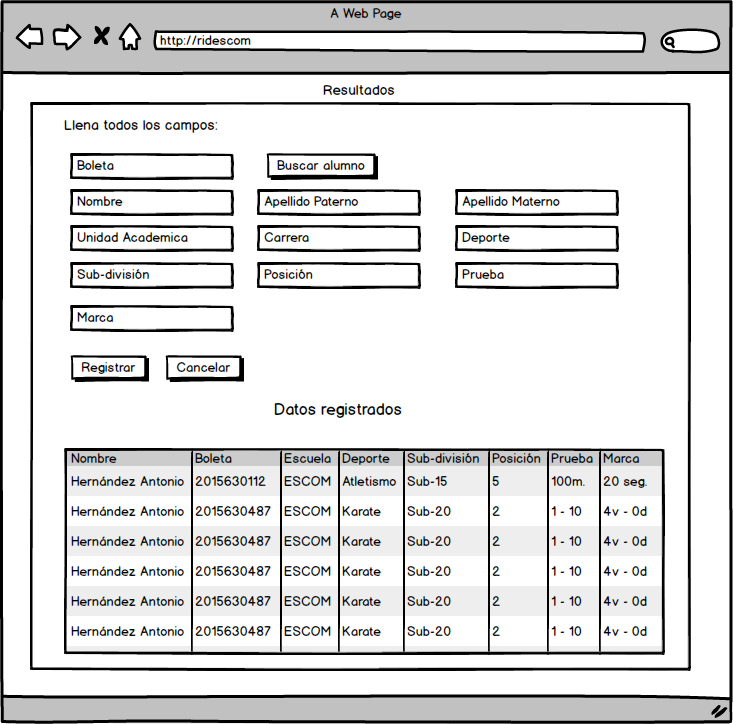
\includegraphics[width=10cm, height=7cm]{Imagenes/Nuevos/P10_Ingresa_resultados}
			\caption{Vista para ingresar los resultados obtenidos por los participantes (Coordinador de Unidad Académica).}
			\label{ingresaresultados}
		\end{figure}
		
		\begin{figure} [hbt!]
			\centering
			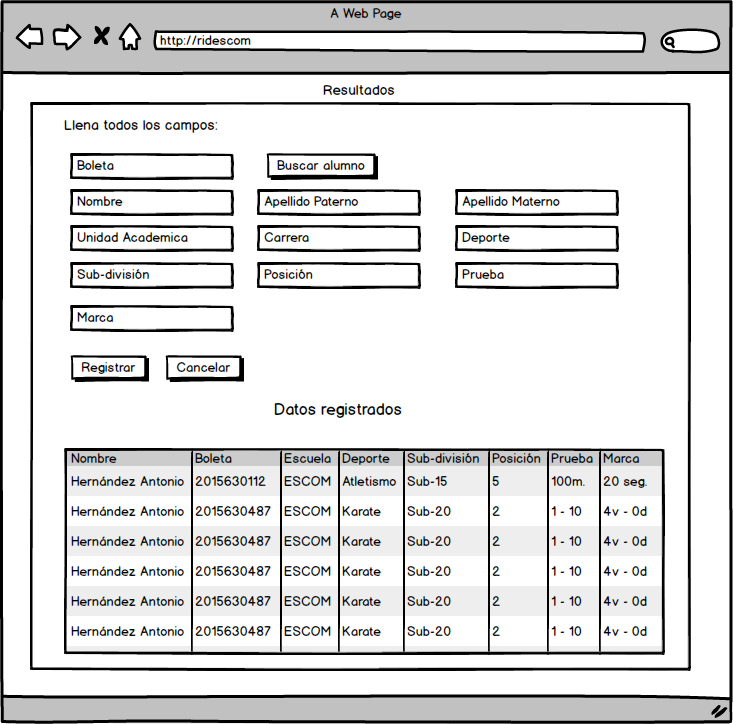
\includegraphics[width=10cm, height=7cm]{Imagenes/Nuevos/P11_Editar_resultados}
			\caption{Vista para editar los resultados de los participantes (Coordinador de Unidad Académica).}
			\label{editaresultados}
		\end{figure}
		\pagebreak
		
		\begin{figure} [hbt!]
			\centering
			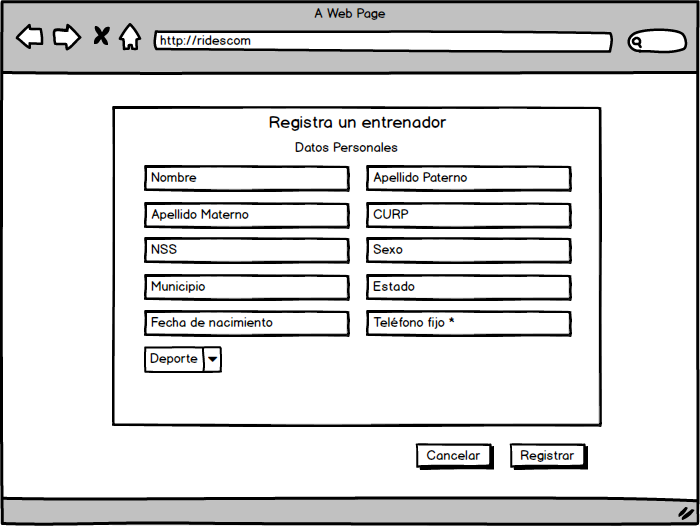
\includegraphics[width=10cm, height=6cm]{Imagenes/Nuevos/P12_Registro_entrenador}
			\caption{Vista para registrar a un entrenador (Coordinador de Unidad Académica).}
			\label{registroentrenador}
		\end{figure}
		
		\begin{figure} [hbt!]
			\centering
			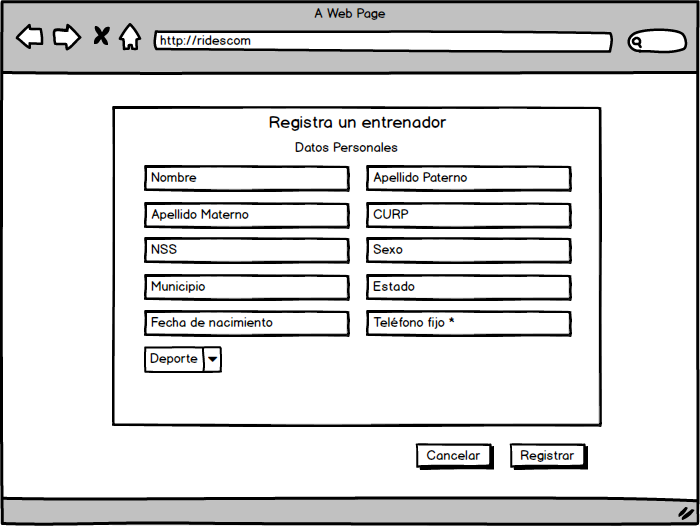
\includegraphics[width=10cm, height=6cm]{Imagenes/Nuevos/P13_Editar_entrenador}
			\caption{Vista para editar los datos del entrenador (Coordinador de Unidad Académica).}
			\label{editarentrenador}
		\end{figure}
		
		\begin{figure} [hbt!]
			\centering
			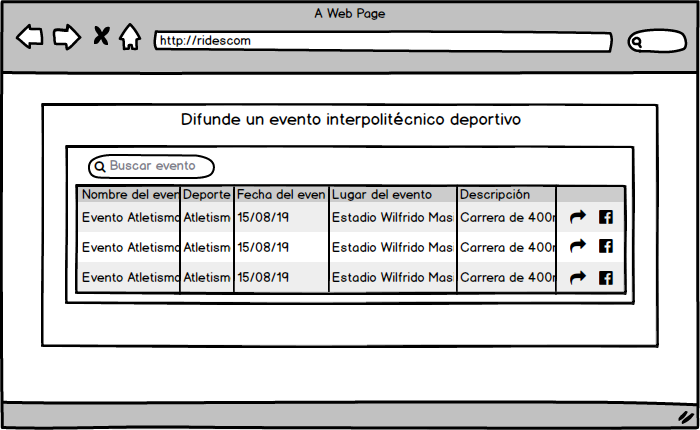
\includegraphics[width=10cm, height=6cm]{Imagenes/Nuevos/P14_Difundir_evento}
			\caption{Vista para difundir un evento interpolitécnico deportivo (Coordinador de Unidad Académica).}
			\label{difundirevento}
		\end{figure}
		\pagebreak

		\begin{figure} [hbt!]
			\centering
			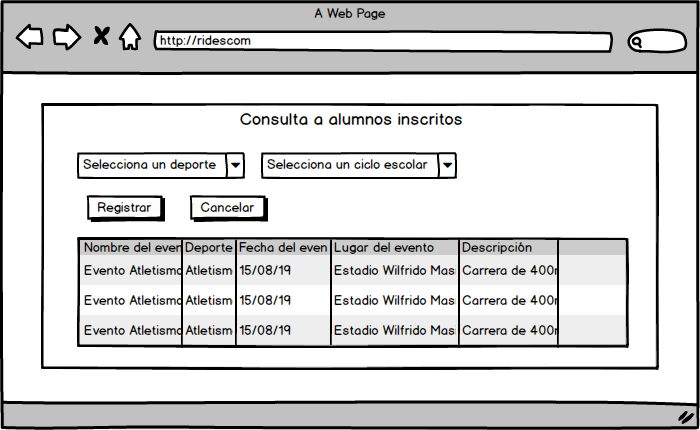
\includegraphics[width=10cm, height=6cm]{Imagenes/Nuevos/P15_Consulta_alumnos_inscritos}
			\caption{Vista para consultar los alumnos que se han inscrito a un evento (Coordinador de Unidad Académica).}
			\label{consultaalumnosinscritos}
		\end{figure}
	
		\begin{figure} [hbt!]
			\centering
			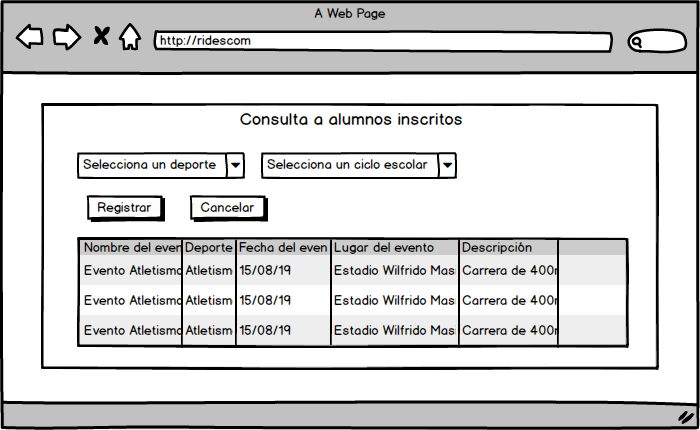
\includegraphics[width=10cm, height=6cm]{Imagenes/Nuevos/P16_Consulta_para_expedir_constancias}
			\caption{Vista para consultar participación de alumnos (Coordinador).}
			\label{consultaparaexpedirconstancias}
		\end{figure}
		
		\begin{figure} [hbt!]
			\centering
			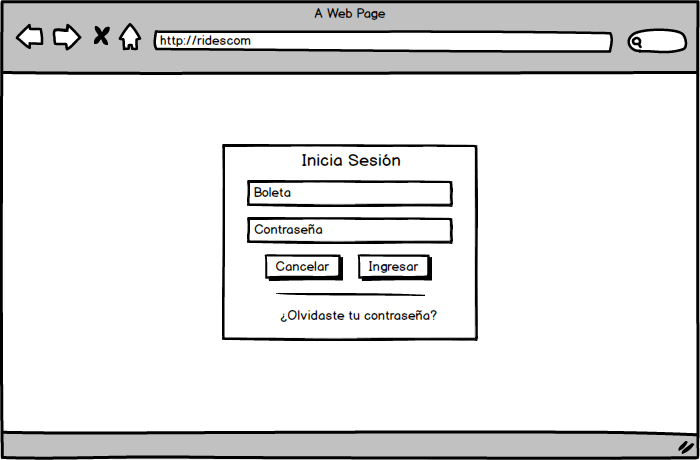
\includegraphics[width=10cm, height=6cm]{Imagenes/Nuevos/P17_Login_alumno}
			\caption{Vista Inicio de Sesión para el alumno.}
			\label{loginalumno}
		\end{figure}
	\pagebreak
		
		\begin{figure} [hbt!]
			\centering
			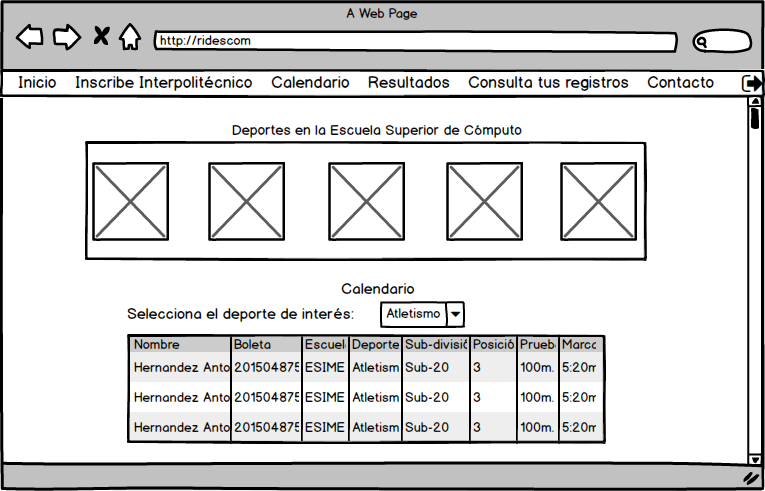
\includegraphics[width=10cm, height=6cm]{Imagenes/Nuevos/P18_Inicio_paticipante}
			\caption{Vista principal del alumno.}
			\label{principalalum}
		\end{figure}
		
		\begin{figure} [hbt!]
			\centering
			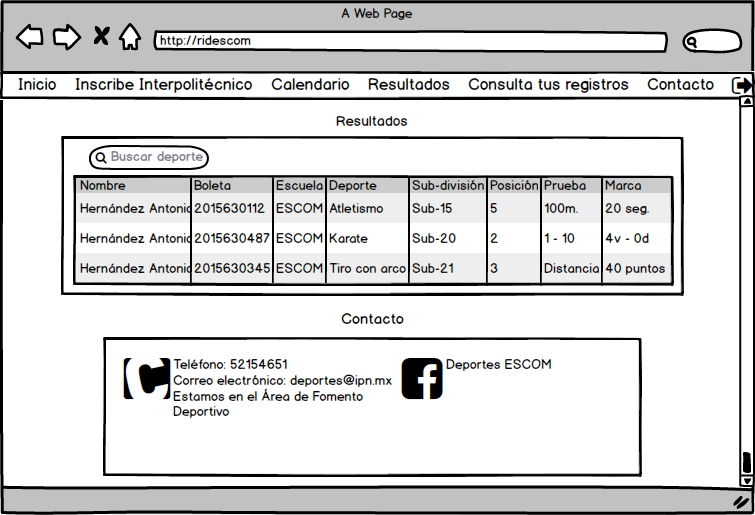
\includegraphics[width=10cm, height=6cm]{Imagenes/Nuevos/P19_Inicio_paticipante1}
			\caption{Vista principal del alumno (Continuación).}
			\label{principalalum1}
		\end{figure}
	
		\begin{figure} [hbt!]
			\centering
			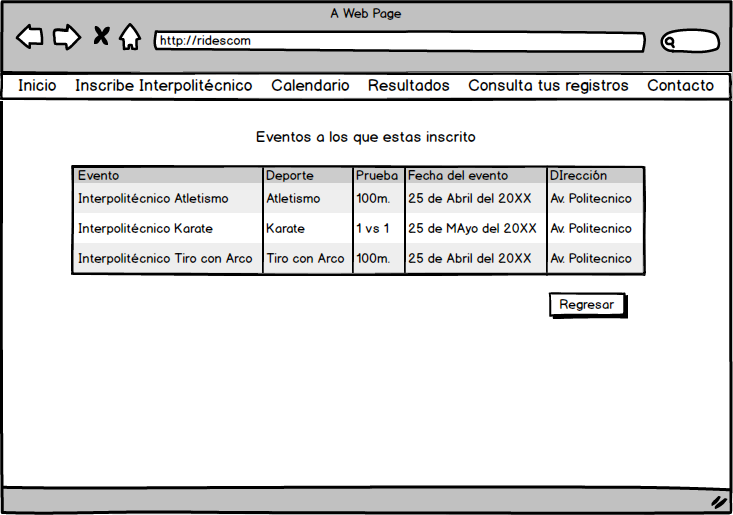
\includegraphics[width=10cm, height=6cm]{Imagenes/Nuevos/P20_Consulta_Inscripciones}
			\caption{Vista para consultar los eventos a los que se a registrado el alumno (Alumno).}
			\label{consultainscripcion}
		\end{figure}
	\pagebreak
		
		\begin{figure} [hbt!]
			\centering
			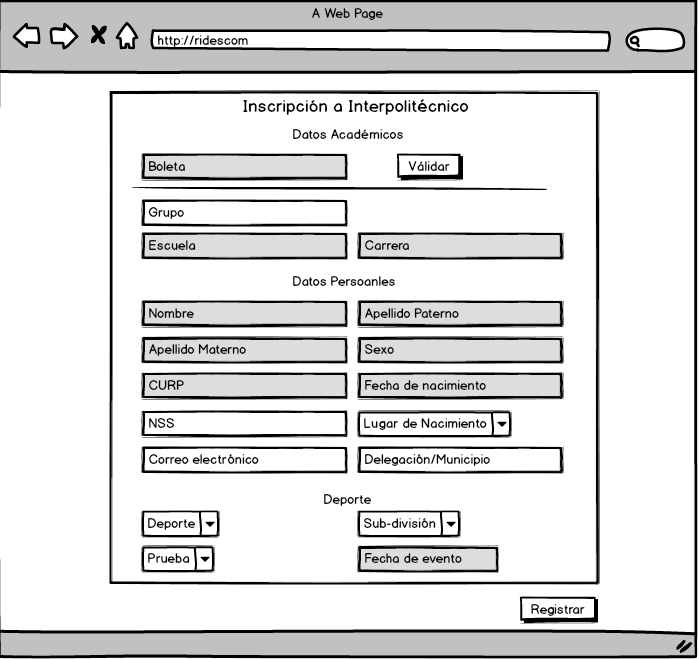
\includegraphics[width=10cm, height=6cm]{Imagenes/Disenos/Inscripcioninter}
			\caption{Formulario para que el alumno se registre en un evento interpolitécnico deportivo.}
			\label{Inscripcioninterpolitecnico}
		\end{figure}
		

		\begin{figure} [hbt!]
			\centering
			\inputgraphics[width=10cm, height=6cm]{Imagenes/Nuevos/P21_Historial}
			\caption{Vista para que el alumno pueda visualizar todos los eventos en los que ha participado.}
			\label{historial}
		\end{figure}